\section{Evaluierung}
Im folgenden Kapitel werden alle Phasen einer durchgeführten Studie zur Evaluation der Eignung eines IT-gestützten Trainings beschrieben. Die Studie bestand aus folgenden Phasen: Vorarbeitungphase, Entwurfsphase, Rekrutierungsphase, Studienphase, Nacharbeitung der Ergebnisse und Evaluation.

\paragraph{Das Ziel der Studie} ist eine Evaluierung der Eignung des Mimikry Trainings. Unter dem Begriff "Eignung" werden im Zuge dieser Arbeit vor allem die User Expierience (UX) Aspekte gemeint, wie Nutzerfreundlichkeiteit der Software oder Usability (siehe Kapitel 1 Motivation und Kapitel 2 Grundlagen).

Die primäre Zielgruppe für diese App sind Menschen mit einer Autismus Diagnose und/oder mit Emotionserkennungsdefiziten. Ältere Menschen oder Menschen aus fremden Kulturkreisen, die Deutsch gut beherrschen, können als sekundäre Zielgruppe gesehen werden.

\subsection{Vorarbeitungsphase}
Während der Vorarbeitungsphase wurden verschiedene Fragebögen untersucht: ISONorm 110, ISOMetrics, AttrakDiff, User Experience Questionnaire, QUIS, SUMI. Es wurden Fragebögen gewählt, die eine Eignung des computergestützten Trainings nach der im Kapitel 1 genannten Definition bewerten könnten. Primär wurde der UEQ Fragebögen(siehe Kapitel 2, Grundlagen) zur Abschätzung folgender Variablen gewählt: Attraktivität, Durchschaubarkeit, Effizienz, Steuerbarkeit, Stimulation, Originalität.  Es wurde zusätzlich der SUS(siehe Kapitel 2, Grundlagen), Fragebogen zur Abschätzung der Gebrauchstauglichkeit der Software ausgewählt. Beide Fragebögen sind frei zugänglich und haben haben sich als zuverlässig erwiesen. Sie bieten einen Qualitätsvergleich mit einer großen Probe von auf dem Markt bereits existierenden Software.

\subsection{Entwurfsphase}
Während der Entwurfsphase wurden folgende Entscheidungen getroffen:
Die Studie wird mittels eines quantitativen Vorgehens entworfen, mit zusätzlichen optionalen qualitativen Fragen, bei besonders positiv oder negativ ausgefallenen Antworten.
Es gibt sehr viele quantitativen Methoden, um unterschiedliche Variablen zur Evaluation bewerten zu können. Für den Zweck dieser Studie wurden der User Experience Questionnaire UEQ~\cite{UEQ} und der System Usability Scale (SUS)~\cite{SUS} Fragebogen ausgewählt.
\subsubsection{Ablauf der Studie}
Während der Studie werden die Probanden beobachtet, um allen möglichen Störungen, die aufgetreten könnten, zu protokollieren. Es wird zusätzlich der qualitative Aspekt der Studie berücksichtigt. Die Probanden sollten unabhängig in unterschiedlichen Räumen mit ähnlichen Rahmenbedingungen getestet werden. 
Jedes mal vor dem Spielen wird der Sinn von einem computergestützten Training im Bezug auf Autismuspatienten erklärt, so dass die Probanden ein ähnliches Wissen wie die zukünftigen Nutzer haben. 
Mimikry wurde mit einem zu dem Rest der App kohärenten Design entwickelt. Dieses Design unterscheidet sich leicht von dem in dem Material Design beschriebenen Standarten - es treten ungewöhnliche Knöpfe und Balken auf, was einen Einfluss auf das UX und Usability haben könnte. Mimikry sollte auch als eines letzten Module trainiert werden, wo man sich bereits mit den untypischen Bedienungen am Beispiel der früheren Modulen vertraut machen konnte. Die bisher existierenden Module der ''E.V.A'' App werden den Probanden beschrieben, so dass das Mimikry Modul nicht als eine separate App sondern ein separates Modul wahrgenommen werden konnte. 
Der Ablauf des Spiels wird in dem Abschnitt ''Ablauf des Spiels'' ausführlich beschrieben.
Nach der Interaktion mit dieser App sollten die Probanden einen Online-Fragebogen ausfüllen, der aus zwei Teilen besteht: User Experience und Usability. Durch das Anwenden der Google Forms werden die Ergebnisse sowohl in dem CSV Format als auch in der Form von Diagrammen direkt verfügbar. 
Die Antworten, die besonders positiv oder negativ ausgefallen sind werden beschrieben.

\subsubsection{UEQ - eine Methode zur Evaluation von User Experience}
Der UEQ Fragebogen besteht aus 26 Fragen, die Gegensatzpaaren von Eigenschaften zur Beschreibung der Interaktion mit der App abbilden. Um den empirischen Aspekt der Studie zu berücksichtigen wird es empfohlen, die Evaluation möglichst direkt nach der Nutzung der Software durchzuführen.
In der Umfrage wird der Nutzer darum gebeten, das Produkt zu bewerten. Um die Missverständnisse zu vermeiden, wird der Begriff ''Produkt'' mit den Begriffen ''App'' oder ''Spiel'' ersetzt.

Es werden folgende Variablen evaluiert: 
\begin{enumerate}
    \item Attraktivität: Allgemeiner Eindruck. Mögen die Nutzer die App?
    \item Bedienungsfreundlichkeit: Ist es einfach sich mit der App vertraut zu machen?
    \item Effizienz: Können die Nutzer das Training durchführen, ohne sich anstrengen zu müssen?
    \item Zuverlässigkeit: Hat der Nutzer die Kontrolle über Interaktionen?
    \item Stimulation: Wird der Nutzer durch Interaktionen mit der App motiviert?
    \item Neuartigkeit: Ist die App innovativ?
\end{enumerate}
 Abstufungen zwischen den Gegensätzen sind durch Kreise dargestellt. Durch Ankreuzen einer dieser Kreise können die Nutzer die Stärke ihrer Zustimmung zu einem Begriff äußern. 
Der Fragebogen untersucht das Nutzungserlebnis hinsichtlich der Faktoren Attraktivität, Durchschaubarkeit, Effizienz, Steuerbarkeit, Stimulation und Originalität. Das zugehörige Auswertungstool beinhaltet einen Benchmark-Datensatz zu Softwareprodukten aus 246 Studien mit 9905 Testpersonen, zu denen die Mittelwerte der eigenen Studien in Relation gesetzt werden~\cite{ueqpublication}.

\subsubsection{SUS - eine Methode zur Evaluation von Usability}
Die SUS Scale ist ein Fragebogen zur Messung der Gebrauchstauglichkeit eines Systems.  Die Antworten werden mittels einer typischen Likert-Skala ermittelt~\cite{ Jordan1996}. Es wird aus den Antworten eine Punktzahl zwischen 0 und 100 berechnet. Diese Zahl misst die Usability der untersuchten Software. Ab 68 Punkten gelten Ergebnisse als zufriedenstellend gemäß Usability und die Software kann als gebrauchstauglich bezeichnet werden.~\cite{SUS}\textsuperscript{,}~\cite{ Jordan1996}. Der Fragebogen ist technologie-unabhängig und besteht aus folgenden 10 Aussagen~\cite{SUS_online}.
\begin{enumerate}
    \item Ich kann mir sehr gut vorstellen, das System regelmäßig zu nutzen.
    \item Ich empfinde das System als unnötig komplex.
    \item Ich empfinde das System als einfach zu nutzen.
    \item Ich denke, dass ich technischen Support brauchen würde, um das System zu nutzen.
    \item Ich finde, dass die verschiedenen Funktionen des Systems gut integriert sind.
    \item Ich finde, dass es im System zu viele Inkonsistenzen gibt.
    \item Ich kann mir vorstellen, dass die meisten Leute das System schnell zu beherrschen lernen.
    \item Ich empfinde die Bedienung als sehr umständlich.
    \item Ich habe mich bei der Nutzung des Systems sehr sicher gefühlt.
    \item Ich musste eine Menge Dinge lernen, bevor ich mit dem System arbeiten konnte.
\end{enumerate}

\paragraph{Weitere potenziellen Variablen zur Evaluierung.}Weitere Aspekte, wie die Qualität des Flows (also wie engagiert die Benutzer sind, was eine sehr große Rolle bei dem Game-Based Learning spielt) oder die Lernrate des Emotionen Nachahmungseffekts, sind auch potentiell messbar, aber das Hinzufügen von weiteren Methoden würde die Komplexität der Studie deutlich erhöhen und folglich den Umfang der Aufgabenstellung dieser Arbeit überschreiten. Weil der Flow eher im Zusammenhang mit dem gesamten E.V.A. Spiel steht, wurde er bei dieser Studie weggelassen. Die Lernrate des Emotionen Nachahmungseffekts ist für die Untersuchung der Eignung nicht relevant um komplexer zu untersuchen.

\paragraph{Rekrutierungsphase und Beschreibung der Probandengruppe}  Aufgrund der spezifischen Zielgruppe ist es schwierig, eine Studie ausschließlich mit solchen Probanden durchzuführen, wenn man nicht direkt mit Ihnen arbeitet. Trotz der Schwierigkeiten wurde ein passender Proband mit einer Autismus Diagnose gefunden. Die Studie mit ihm und den restlichen 19 Probanden (davon 6 weibliche und 14 männliche) sorgten dafür, dass die Ergebnisse zuverlässiger sind und die Eignung des Trainings getestet werden konnte. Die Versuche ältere Menschen für die Studie zu finden waren nicht erfolgreich (ein potenzieller Proband hat die Teilnahme wegen der moralischen Seite der künstlichen Intelligenz verweigert). 2 Probanden kommen aus dem Ausland, die Länder hatten aber eine ähnliche Kultur wie Deutschland und es wurden bei den Personen kein ungewöhnliches Verhaltensmuster beobachtet. Das Alter in der Gruppe betrug von 18 bis 35 Jahren. Die Gruppe bestand zum großen Teil aus wissenschaftlichen Mitarbeiter*innen und Student*innen von Informatik und Wirschaftsinformatik.

\subsection{Verlauf der Studie}
Das Spiel bestand aus einem kurzen Interview vor dem Test, in dem die Probanden Angaben zur Autismus-Diagnose und dem Alter gemacht haben. Ich habe das Konzept von E.V.A. und die Spielspezifischestruktur - Einführungstutorials, das Spiel selbst und Feedbackscreens erklärt, siehe \ref{einf}.

\subsubsection{Ablauf des Spiels}Die Probanden bekommen als erstes ein Screen mit dem Einführungstutorial angeziegt (sehe Implementierung: Einführungstutorial: MimicryPreviewIntro). Danach erschien die Aufgabe. Die Probanden sollten die vorgegebene Emotion 15 Sekunden lang nachahmen. Aufgrund der Erhöhung der Reliabilität der Messergebnisse, die in der Datenbank für die zukünftigen Arbeiten verwendet werden könnten, wird jede Emotion in beiden Varianten (mit und ohne Vorschau, siehe Implementierung) getestet. Die Einführungstutorials wurden nur ein mal, vor dem ersten Spielen jeweiliger Variante dargestellt. Nachdem die Zeit abgelaufen war haben die Nutzer das Feedback bekommen, ob die Aufgabe gelöst wurde oder nicht. Nachdem die beiden Spielvarianten mit jeweils vier Emotionen gespielt wurden, haben die Probanden den Fragebogen auf einem Laptop ausgefüllt.

Während der Studienphase wurden alle Bemerkungen von den Benutzern und zusätzliche Beobachtungen notiert, was ausführlich in dem nächsten Abschnitt beschrieben wird.

\subsubsection{Nachbereitung von Daten}
Beide Fragebögen wurden separat mit Hilfe von den vorgefertigten Microsoft Excel Templates analysiert. Nachdem die gesammelten Daten eingegeben wurden, wurde der erste Schritt der Analyse durchgeführt. Der zweite Schritt bestand aus der Analyse von erzeugten Diagrammen und gesammelten Beobachtungen.

Die Aussagen und Bemerkungen, die während der Studie gesammelt wurden, wurden ich in einem separaten Anhang gesammelt, vgl. \ref{quailtat}, \ref{knopf}, \ref{winkel}. Sie werden ebenso in dem nächsten Abschnitt beschreiben
\subsection{Ergebnisse der Studie} 
Das Modul wurde bezüglich der Usability und User Experience als sehr gut bewertet. 
Das Ergebnis des Usability Fragebogens beträgt 83.8 was eine nutzerfreundliche Software kennzeichnet~\cite{Usability}.
In dem zweiten Teil der Studie wurde die User Experience gemessen, siehe Abb.\ref{uxmimikry}, der Fragebogen ist im Appendix \ref{ueq} enthalten.
\begin{figure}[H]
\centering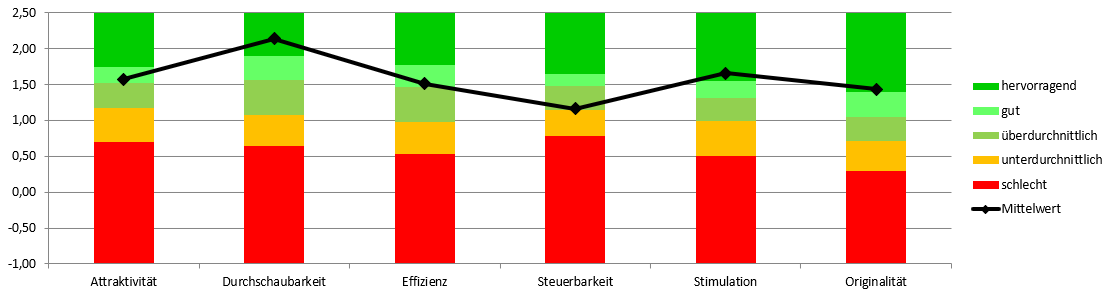
\includegraphics[width=330pt]{res/ux_final}
\caption{Ergebnisse der User Experience Studie}
\label{uxmimikry}
\end{figure}

Die Probanden waren mit dem Design und der visuellen Seite der App sehr zufrieden. 14 haben das Mimikry Modul als attraktiv oder sehr attraktiv bewertet.
17 Probanden fanden das Mimikry Modul sympathisch oder sehr sympathisch. Sieben Probanden haben ein zusätzliches, positives mündliches Feedback zu dem Modul geäußert(siehe Appendix, ref. \ref{quailtat}).

User Experience wurde als hervorragend auf der Durschubarkeit-, Stimulation- und Originalität- Skala, als gut auf der Attraktivität- und Effizienz-Skala und über dem Durchschnitt auf der Steuerbarkeits-Skala bewertet. (siehe Abb.\ref{uxmimikry}). 

Die Probanden haben das Design als (siehe Abb.\ref{uxmimikry_detailed}.) ‘übersichtlich’ und ‘leicht zu lernen’ (M = 2,4) empfunden, was den Gesamtwert der Durchschaubarkeit-Skala hochsetzte. Das Spielerlebnis wurde als sehr ‘effizient’ (M = 2,3) bewertet. Das höchste Ergebnis auf der Stimulation-Skala wurde durch den Item ‘interessant’ erreicht (M = 2,1). Hinsichtlich Attraktivität ist das Item ‘sympathisch’ (M = 2,1) am stärksten ausgefallen. Alle Items der Originalität-Skala haben ähnliche Werte, leicht über dem Durchschnitt erreicht (~M = 1,5).

\begin{figure}[H]
\centering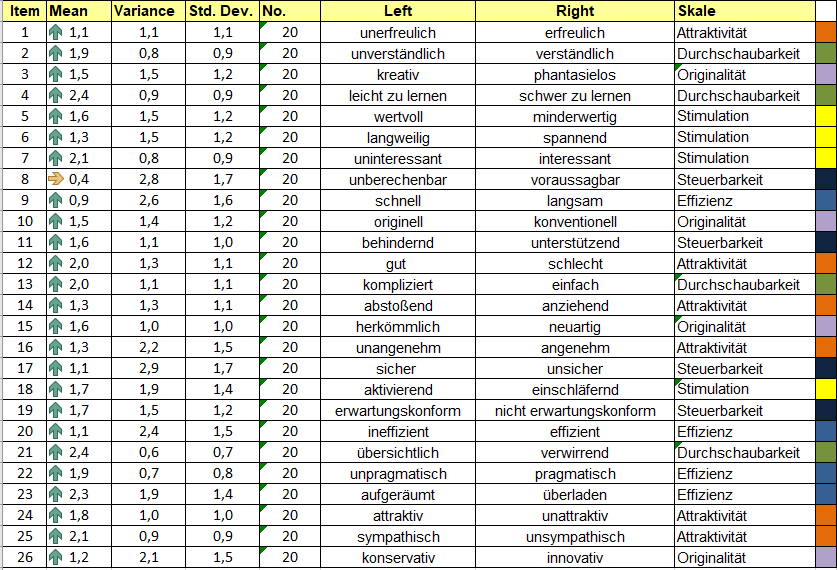
\includegraphics[width=360pt]{res/ueq_detalliert}
\caption{Ergebnisse der User Experience Studie. Die 8. Variable, ''unberechenbar/voraussagbar'' wurde am schlechtesten bewertet (Mittelwert = 0,4; Standardabweichung = 1,68; Varianz = 2.8). Die Probanden bei diesem Punkt nicht einig siehe Abb.\ref{item_8}. Durchschaubarkeit bei Variablen 4 (M = 2,4; SD = 0.9,68; V = 0.9) und 21 (M = 2.4; SD = 0.7; V = 0.6) wurden sehr positiv bewertet siehe Abb.\ref{item_4}, Abb.\ref{item_21}}
\label{uxmimikry_detailed}
\end{figure}
Konkret haben die Probanden das Mimikry Modul zum Teil als unberechenbar bewertet vgl. Abb. \ref{uxmimikry_detailed},  Abb.\ref{item_8}, was die Steuerbarkeit beeinflusste. 
Die qualitative Evaluation hat aufgezeigt, dass Mimikry inkonsistente Stellen beinhaltete. Konkret wurde die Verwendung der Navigationselemente bei der Variante ohne Vorschau als unvorhersehbar bewertet. Bei der gleichen Variante wurde Imitation als intransparent empfunden.
Es gab zwei Stellen an denen die Steuerbarkeit verbessert werden könnte. (siehe Appendix, ref.\ref{quailtat}) \\
Viele Probanden fühlten sich unsicher bei der Mimikry Variante ohne Vorschau. Sie waren sich nicht sicher, ob sie bei 0\% bleiben, weil die Zielemotion gerade falsch nachgeahmt wird oder vielleicht befindet sich das Gesicht gerade außerhalb dem Kamerafeld. Die Unterschiede werden an keiner Stelle markiert. 
Die Unsicherheit beim Steuern führte bei fast allen Probanden zu einer leichten Frustration und es ist definitiv ein Faktor, der zu vermeiden ist. 14 Probanden haben ihre Meinung dazu spontan geäußert. Sie haben sich gewünscht, zu wissen, ob sie sich innerhalb von einem Kamerafeld befinden.\\
Der zweite Ansatzpunkt für mögliche Verbesserungen ist bei der Mimikry Variante ohne eine Vorschau, bei der die Zielemotion für 10 Sekunden präsentiert wird. Danach erscheint automatisch die Zielaufgabe. Während dieser Phase hätte der Faktor von Kohärenz stärker ausgeprägt sein können. 
Folgendes wurde durch das Beobachten von den Probanden bei dem Spielen herausgefunden.
10 Probanden haben versucht, den Schritt zu überspringen und haben nach einem Knopf gesucht, der die eigentliche Aufgabe starten könnte. Sieben haben sogar die Fläche, wo er sein könnte, angeklickt. Fünf Probanden haben sich nach dem Spielen gewünscht, diese Möglichkeit zu haben. Neun Probanden haben zusätzlich berichtet, sie würden gerne die Mechanismen hinter der Aufgabenbewertung besser verstehen. 
Die Fragebögen wurden von den Benutzern direkt nach dem Spielen ausgefüllt.

\subsubsection{In der Studie festgestellten Verbesserungsvorschläge}
Es gab zwei Stellen wo man die Steuerbarkeit verbessern könnte. \\
Viele Probanden fühlten sich unsicher bei der Mimikry Variante ohne Vorschau. Man ist sich nicht sicher, ob man bei 0\% bleibt, weil die Zielemotion gerade falsch nachahmt wird oder vielleicht befindet sich das Gesicht gerade außer dem Kamerafeld. Es wird an keiner Stelle markiert. 
Die Unsicherheit beim Steuern führte bei fast allen Probanden zu einer leichten Frustration. Dieser Faktor ist unter der Beachtung von Game Based Learning Prinzipien zu vermeiden. 14 Probanden haben ihre Meinung dazu spontan geäußert und sich gewünscht, kontinuierlich zu wissen, ob sie sich innerhalb von einem Kamerafeld befinden.\\
Die zweite Stelle für möglichen Verbesserungen ist bei der Mimikry Variante ohne eine Vorschau, wo die Zielemotion für 10 Sekunden präsentiert wird zu sehen, bevor es automatisch zu der eigentlichen Aufgabe gewechselt wird. Während dieser Phase hätte der Faktor von Kohärenz stärker ausgeprägt sein können. Folgendes wurde durch das Beobachten von den Probanden bei dem Spielen herausgefunden. 10 Probanden haben versucht, den Schritt in dem die Zielemotion präsentiert wird zu überspringen und haben nach einem Knopf gesucht, der die eigentliche Aufgabe starten könnte. Sieben Probanden haben sogar die Fläche, wo der Knopf sein könnte angeklickt. Fünf Probanden haben sich nach dem Spielen es auch gewünscht, diese Möglichkeit zu haben.

Die Verbesserung der Transparenz der Aufgabenbewertung. Nach dem GBL Prinzipien sollte man versuchen, die Software transparent und intuitiv zu gestalten (siehe Kapitel 2, Grundlagen)~\cite{Prensky2003DigitalGL}. Eine mögliche Lösung des Problems wäre Implementierung zusätzlicher Elementen bei den Tutorials. Es könnte jedoch die Überschaubarkeit negativ beeinflussen.

\subsubsection{Die Meinung des Probanden mit einer Autismus Diagnose}
Der einzige Proband mit einer Autismus Diagnose aus der Gruppe hat sehr viele Interessante Bemerkungen getätigt. Seines Erachtens nach ist die App für ihn nicht besonders nützlich, weil er gewohnt ist, immer eine Begleitperson dabei zu haben. Die Begleitperson betreut ihn fast ständig und leistet Hilfe in sozialen und beruflichen Situationen. Wegen der fast ständigen Anwesenheit von der Begleitperson ist für ihn persönlich die App nicht erforderlich. An der Stelle wurde dem Probanden eine Frage dazu gestellt. Er war in der Lage, sich eine Situation vorzustellen, in der diese Betreuung nicht anwesend wäre. In dieser Situation könnte er sich vorstellen, von der Nutzung unserer Software zu profitieren.\\
Das führt schließlich dazu, dass man selbständiger im Alltag wird und es war ein sehr interessantes Erkenntnis aus der Studie.

\subsection{Evaluation der Eignung des Trainings des Mimikry Moduls}
Zu Evaluation der Eignung werden UX und Usability untersucht.
Aus der Perspektive lässt sich schließen, dass die Entscheidung das Mimikry Moduls in zwei möglichen Spielszenarien zu implementieren sehr gut getroffen war.  
Der gesamt Eindruck des Spiels bezüglich dem User Experience und Usabililty ist ausreichend, um von einer guten Eignung des computergestützten Trainings reden zu können. Aus den zwei Modulen hat sich besonders die Mimikry Variante mit Vorschau als nutzerfreundlich herausgestellt. Die zweite Variante benötigte eine Anpassung, was sich mit der existierenden Software leicht umsetzen lässt, zum Beispiel im Form eines grünen/roten Hintergrunds (was aber nicht  bei einer bestehenden Rot-Grün-Sehschwäche geeignet wäre), je nachdem ob man von der Kamera erfasst wird.



